\chapter{Táticas Elementares}

\section{Escadas}

Escadas constituem uma das técnicas mais básicas\footnote{Uma técnica ser básica não garante que ela seja fácil de dominar. Mesmo profissionais encontram posições de escadas difíceis e complicadas em suas partidas.} de captura. Elas também são mais do que uma técnica local, dado que requerem consciência das condições no resto do tabuleiro.

\emph{Dia.\@~1.} A pedra preta marcada está cortando Branco em dois grupos, então Branco gostaria de capturá-la. Como ele poderia fazê-lo?

\emph{Dia.\@~2.} Começa-se pelo atari em 1.

\begin{figure}[h!]
    \centering
    \begin{subfigure}[t]{.3\textwidth}
        \centering
        
\includegraphics[width=.9\textwidth]{7 - Ladders - Dia 1}
        \captionsetup{justification=centering}
        \caption*{\emph{Dia.\@~1}}
    \end{subfigure}
    \hfill
    \begin{subfigure}[t]{.3\textwidth}
        \centering
        
\includegraphics[width=.9\textwidth]{7 - Ladders - Dia 2}
        \captionsetup{justification=centering}
        \caption*{\emph{Dia.\@~2}}
    \end{subfigure}
    \hfill
    \begin{subfigure}[t]{.3\textwidth}
        \centering
        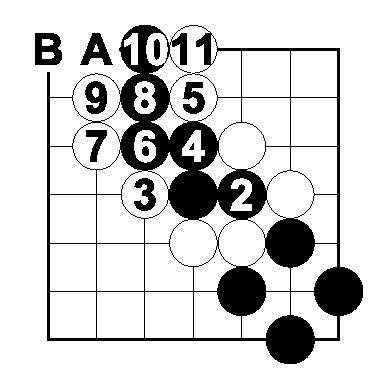
\includegraphics[width=.9\textwidth]{7 - Ladders - Dia 3}
        \captionsetup{justification=centering}
        \caption*{\emph{Dia.\@~3}}
    \end{subfigure}
\end{figure}

\emph{Dia.\@~3.} Se Preto tentar escapar, Branco continua com os ataris de 3 a 11 até onde Preto esgota suas possibilidades. Se Preto \textbf{A}, Preto ainda estará sob atari, então Branco poderá ignorar tal jogada. Assim que as pedras brancas entrarem em perigo, Branco poderá capturar em \textbf{B}. Esse tipo de sequência, na qual o inimigo é mantido sob atari e dirigido à borda do tabuleiro, onde ele esgota suas liberdades, é chamado de escada.

\pagebreak

\begin{figure}[h!]
    \centering
    \begin{subfigure}[t]{.4\textwidth}
        \centering
        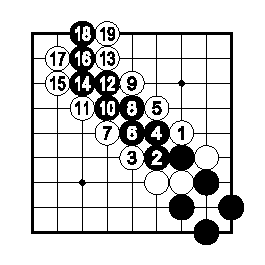
\includegraphics[width=.9\textwidth]{7 - Ladders - Dia 4}
        \captionsetup{justification=centering}
        \caption*{\emph{Dia.\@~4}}
    \end{subfigure}
    \hspace{1cm}
    \begin{subfigure}[t]{.4\textwidth}
        \centering
        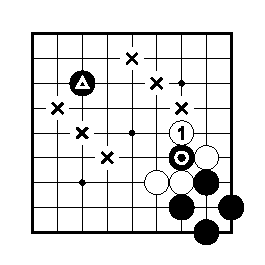
\includegraphics[width=.9\textwidth]{7 - Ladders - Dia 5}
        \captionsetup{justification=centering}
        \caption*{\emph{Dia.\@~5}}
    \end{subfigure}
\end{figure}

\emph{Dia.\@~4.} Aqui está a mesma escada em um tabuleiro maior. São precisos mais movimentos, mas, similarmente, Preto não consegue escapar.

\emph{Dia.\@~5.} Preto possui a pedra triangulada no caminho da escada. O que acontece se Branco tentar capturar, com 1, a pedra circulada?

\emph{Dia.\@~6.} Preto foge com 2. Branco faz atari com 3 a 11, mas, após 12, Preto se conecta com a pedra marcada, ganhando uma liberdade extra. Se Branco continua como anteriormente, Preto agora possui liberdades extras e terá tempo de jogar um duplo-atari em 14. Se Branco conectar com 15, Preto captura uma pedra com 16, colocando outra pedra sob atari. Branco defende com 17, mas Preto pode jogar outro duplo-atari com 18, do outro lado.

\begin{figure}[h!]
    \centering
    \begin{subfigure}[t]{.4\textwidth}
        \centering
        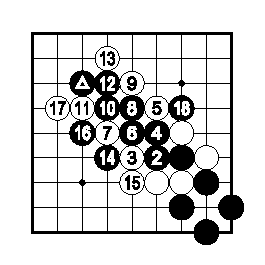
\includegraphics[width=.9\textwidth]{7 - Ladders - Dia 6}
        \captionsetup{justification=centering}
        \caption*{\emph{Dia.\@~6}}
    \end{subfigure}
\end{figure}

Em suma, se Preto possui uma pedra dentro ou em cima do caminho definido pelos pontos $\times$ no \emph{Dia.\@~5}, a escada não será bem sucedida.

Para uma prática adicional sobre escadas, aqui se seguem quatro problemas.

\pagebreak

\subsection{Problemas 31 a 34}

\begin{figure}[h!]
    \centering
    \begin{subfigure}[t]{.35\textwidth}
        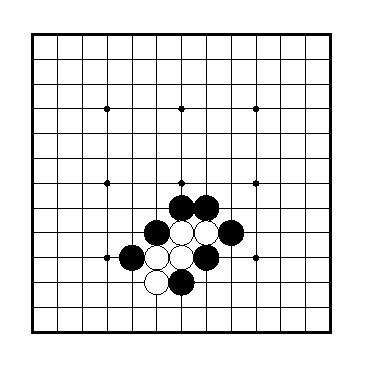
\includegraphics[width=1.25\textwidth]{7 - Problem 31}
        \captionsetup{margin={.15in,0in}}
        \caption*{\textbf{Problema 31}: \emph{Como Preto pode capturar as cinco pedras brancas?}}
    \end{subfigure}
    \hspace{1.5cm}
    \begin{subfigure}[t]{.35\textwidth}
        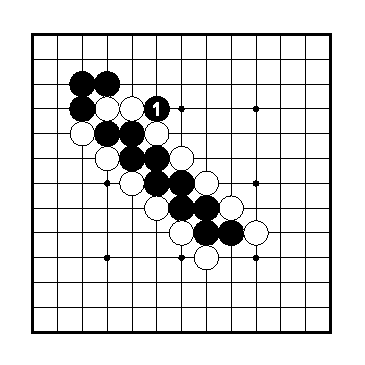
\includegraphics[width=1.25\textwidth]{7 - Problem 32}
        \captionsetup{margin={.15in,0in}}
        \caption*{\textbf{Problema 32}: \emph{Como Branco deveria responder ao duplo-atari preto em 1?}}
    \end{subfigure}
    \par\bigskip
    \par\bigskip
    \begin{subfigure}[t]{.35\textwidth}
        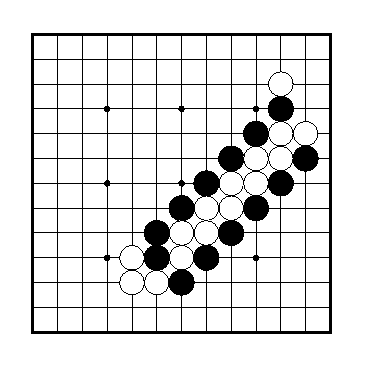
\includegraphics[width=1.25\textwidth]{7 - Problem 33}
        \captionsetup{margin={.15in,0in}}
        \caption*{\textbf{Problema 33}: \emph{Preto possui duas maneiras de fazer atari. Qual é a maneira correta?}}
    \end{subfigure}
    \hspace{1.5cm}
    \begin{subfigure}[t]{.35\textwidth}
        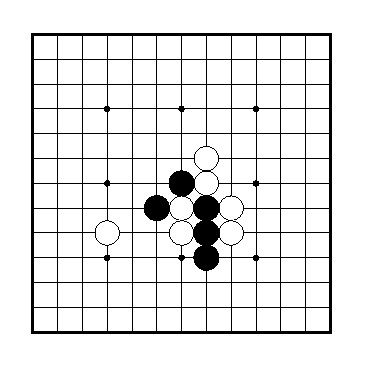
\includegraphics[width=1.25\textwidth]{7 - Problem 34}
        \captionsetup{margin={.15in,0in}}
        \caption*{\textbf{Problema 34}: \emph{Preto possui duas maneiras de fazer atari. Qual é a escolha correta?}}
    \end{subfigure}
\end{figure}

\pagebreak

\subsection{Respostas aos Problemas 31 a 34}

\subsubsection*{Resposta ao Problema 31}

Preto pode capturar as pedras brancas em uma escada com 1 e 3 no \emph{Dia.\@~1}. Depois de Branco 4, Preto direciona as pedras brancas à borda do tabuleiro com 5. Após Preto 7, não há mais nenhuma maneira de Branco evitar ser capturado.

\begin{figure}[h!]
    \centering
    \begin{subfigure}[t]{.425\textwidth}
        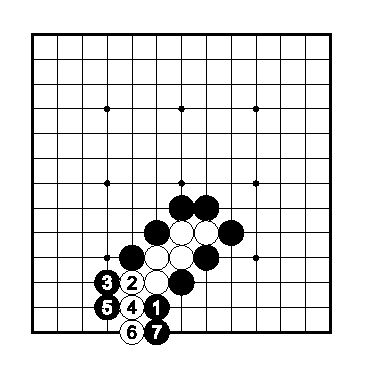
\includegraphics[width=1\textwidth]{7 - Problem 31 - Dia 1}
        \captionsetup{justification=centering}
        \caption*{\emph{Dia.\@~1. Correto}}
    \end{subfigure}
    \hspace{1cm}
    \begin{subfigure}[t]{.425\textwidth}
        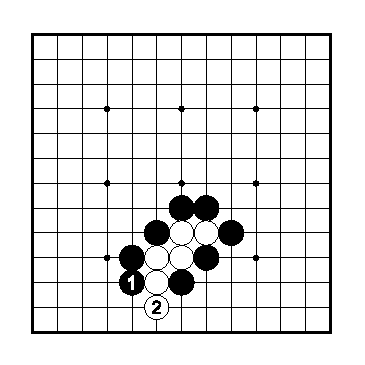
\includegraphics[width=1\textwidth]{7 - Problem 31 - Dia 2}
        \captionsetup{justification=centering}
        \caption*{\emph{Dia.\@~2. Errado}}
    \end{subfigure}
\end{figure}

Preto 1 no \emph{Dia.\@~2} não configura uma escada, então Branco pode aumentar, em duas, suas liberdades descendo para 2. As pedras brancas escapam.

\pagebreak

\subsubsection*{Resposta ao Problema 32}

Branco deveria responder ao duplo-atari de Preto 1 capturando as dez pedras com 2. Isso seria uma perda enorme para Preto.

\begin{figure}[h!]
    \centering
    \begin{subfigure}[t]{.425\textwidth}
        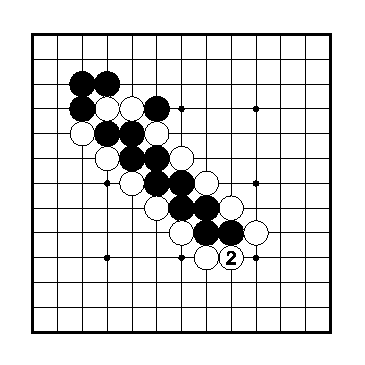
\includegraphics[width=1\textwidth]{7 - Problem 32 - Dia 1}
        \captionsetup{justification=centering}
        \caption*{\emph{Dia.\@~1. Correto}}
    \end{subfigure}
    \hspace{1cm}
    \begin{subfigure}[t]{.425\textwidth}
        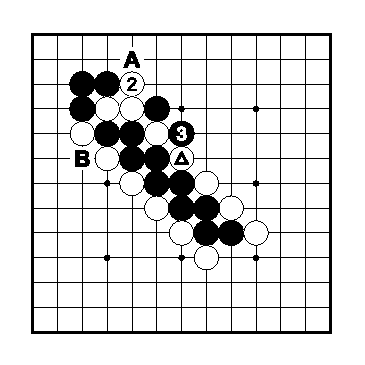
\includegraphics[width=1\textwidth]{7 - Problem 32 - Dia 2}
        \captionsetup{justification=centering}
        \caption*{\emph{Dia.\@~2. Errado}}
    \end{subfigure}
\end{figure}

Se Branco responder a Preto 1 no \emph{Dia.\@~2} tentando resgatar as duas pedras com 2, Preto captura com 3 e ameaça capturar a pedra marcada. Ele também ameaça capturar três pedras em uma escada jogando em \textbf{A}. Preto também possui múltiplas escolhas de duplos-ataris à esquerda, como \textbf{B}.

\pagebreak

\subsubsection*{Resposta ao Problema 33}

Preto deveria dirigir Branco à borda do tabuleiro com o atari de 1 no \emph{Dia.\@~1}. Se Preto fizer atari de novo com 3, não há maneira de Branco sair do atari.

\begin{figure}[h!]
    \centering
    \begin{subfigure}[t]{.425\textwidth}
        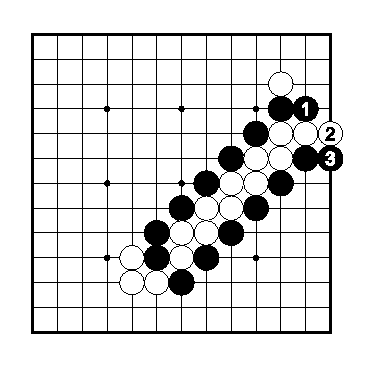
\includegraphics[width=1\textwidth]{7 - Problem 33 - Dia 1}
        \captionsetup{justification=centering}
        \caption*{\emph{Dia.\@~1. Correto}}
    \end{subfigure}
    \hspace{1cm}
    \begin{subfigure}[t]{.425\textwidth}
        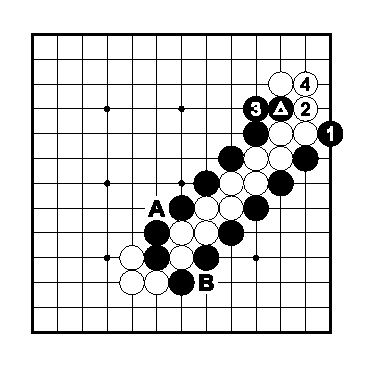
\includegraphics[width=1\textwidth]{7 - Problem 33 - Dia 2}
        \captionsetup{justification=centering}
        \caption*{\emph{Dia.\@~2. Errado}}
    \end{subfigure}
\end{figure}

Jogar o atari na primeira linha com 1 no \emph{Dia.\@~2} é um erro. Branco vira com 2, colocando as pedras marcadas em atari. Preto é forçado a conectar com 3. Ao invés de 4, Branco também pode jogar os duplo-ataris em \textbf{A} e \textbf{B}.

\pagebreak

\subsubsection*{Resposta ao Problema 34}

Preto deveria fazer primeiro atari pela esquerda com 1, então iniciar a escada com 3. A escada agora não colide com a pedra marcada.
        
\begin{figure}[h!]
    \centering
    \begin{subfigure}[t]{.425\textwidth}
        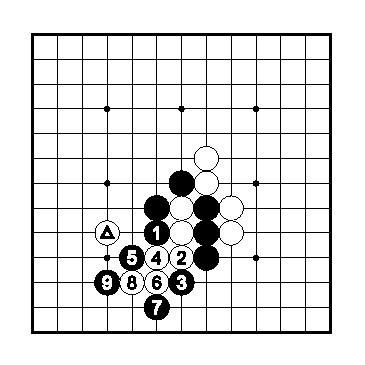
\includegraphics[width=1\textwidth]{7 - Problem 34 - Dia 1}
        \captionsetup{justification=centering}
        \caption*{\emph{Dia.\@~1. Correto}}
    \end{subfigure}
    \hspace{1cm}
    \begin{subfigure}[t]{.425\textwidth}
        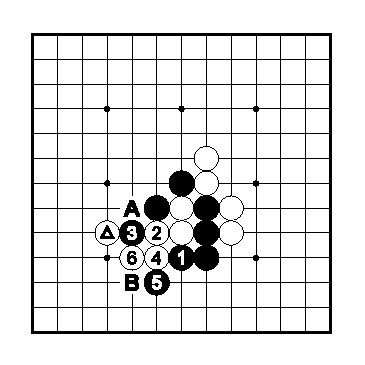
\includegraphics[width=1\textwidth]{7 - Problem 34 - Dia 2}
        \captionsetup{justification=centering}
        \caption*{\emph{Dia.\@~2. Errado}}
    \end{subfigure}
\end{figure}

Se Preto imediatamente começar a escada com a sequência de 1 a 5 no \emph{Dia.\@~2}, devido à presença da pedra marcada, Branco 6 se torna atari na pedra preta em 3. Preto precisa defender conectando em \textbf{A} e, assim, Branco pode jogar \textbf{B}, e suas pedras se salvam.

\pagebreak

\section{Redes}

\emph{Dia.\@~7.} Novamente, Branco quer capturar a pedra marcada.

\begin{figure}[h!]
    \centering
    \begin{subfigure}[t]{.31\textwidth}
        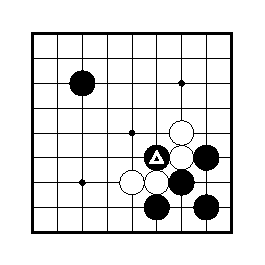
\includegraphics[width=1\textwidth]{7 - Nets - Dia 7}
        \captionsetup{justification=centering}
        \caption*{\emph{Dia.\@~7}}
    \end{subfigure}
    \hfill
    \begin{subfigure}[t]{.31\textwidth}
        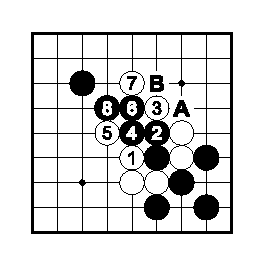
\includegraphics[width=1\textwidth]{7 - Nets - Dia 8}
        \captionsetup{justification=centering}
        \caption*{\emph{Dia.\@~8}}
    \end{subfigure}
    \hfill
    \begin{subfigure}[t]{.31\textwidth}
        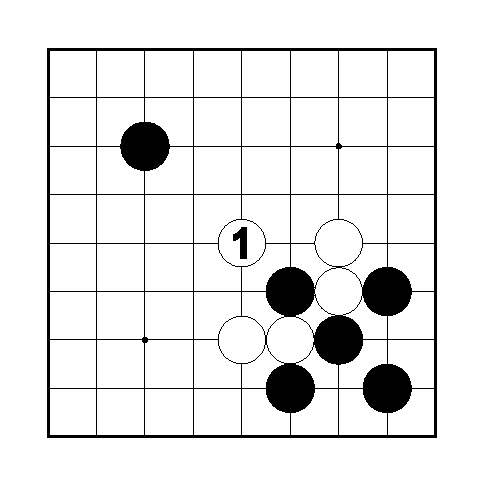
\includegraphics[width=1\textwidth]{7 - Nets - Dia 9}
        \captionsetup{justification=centering}
        \caption*{\emph{Dia.\@~9}}
    \end{subfigure}
\end{figure}

\emph{Dia.\@~8.} Entretanto, a escada correria em uma pedra preta no canto superior esquerdo e colapsaria. Um jogador que tenta uma escada que não funciona, como esta, incorre perdas enormes pois é deixado com vários pontos de corte, como \textbf{A} e \textbf{B} nessa posição. Branco precisa jogar diferentemente.

\emph{Dia.\@~9.} Nesta posição, Branco possui uma alternativa para capturar Preto: é possível contê-lo com 1.

\emph{Dia.\@~10.} Se Preto irrazoavelmente tentar escapar com 2 e 4, Branco capturará com 3 e 5.

\begin{figure}[h!]
    \centering
    \begin{subfigure}[t]{.31\textwidth}
        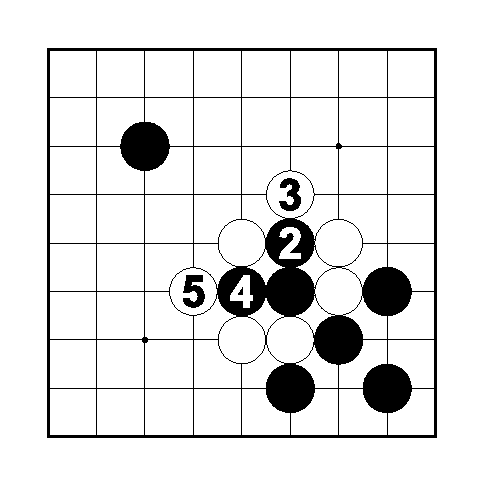
\includegraphics[width=1\textwidth]{7 - Nets - Dia 10}
        \captionsetup{justification=centering}
        \caption*{\emph{Dia.\@~10}}
    \end{subfigure}
    \hspace{1cm}
    \begin{subfigure}[t]{.31\textwidth}
        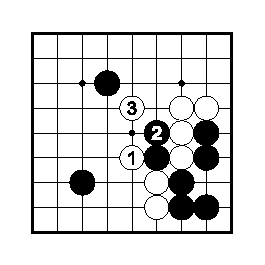
\includegraphics[width=1\textwidth]{7 - Nets - Dia 11}
        \captionsetup{justification=centering}
        \caption*{\emph{Dia.\@~11}}
    \end{subfigure}
\end{figure}

\emph{Dia.\@~11.} Este é outro exemplo de captura com uma rede. Branco pode capturar a pedra marcada jogando primeiro um atari com 1 e, então, enredando-o com 3.

Aqui seguem quatro problemas para se praticar redes.

\pagebreak

\subsection{Problemas 35 a 38}

\begin{figure}[h!]
    \centering
    \begin{subfigure}[t]{.35\textwidth}
        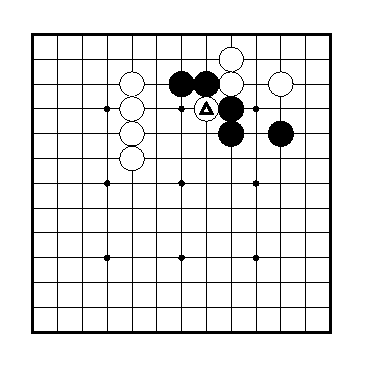
\includegraphics[width=1.25\textwidth]{7 - Problem 35}
        \captionsetup{margin={.15in,0in}}
        \caption*{\textbf{Problema 35}: \emph{Como Preto pode capturar a pedra marcada?}}
    \end{subfigure}
    \hspace{1.5cm}
    \begin{subfigure}[t]{.35\textwidth}
        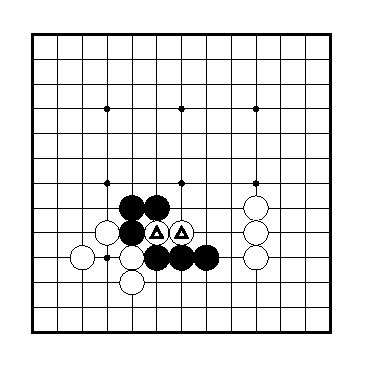
\includegraphics[width=1.25\textwidth]{7 - Problem 36}
        \captionsetup{margin={.15in,0in}}
        \caption*{\textbf{Problema 36}: \emph{Como Preto pode capturar as duas pedras marcadas?}}
    \end{subfigure}
    \par\bigskip
    \begin{subfigure}[t]{.35\textwidth}
        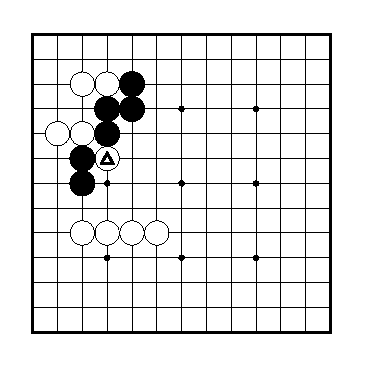
\includegraphics[width=1.25\textwidth]{7 - Problem 37}
        \captionsetup{margin={.15in,0in}}
        \caption*{\textbf{Problema 37}: \emph{Como Preto pode capturar a pedra marcada?}}
    \end{subfigure}
    \hspace{1.5cm}
    \begin{subfigure}[t]{.35\textwidth}
        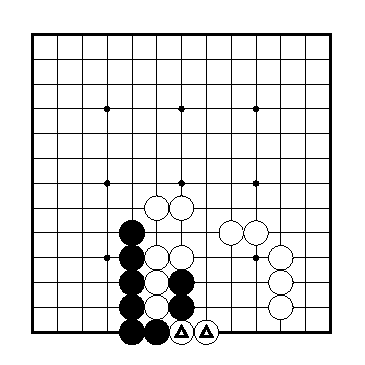
\includegraphics[width=1.25\textwidth]{7 - Problem 38}
        \captionsetup{margin={.15in,0in}}
        \caption*{\textbf{Problema 38}: \emph{Como Preto pode capturar as duas pedras marcadas?}}
    \end{subfigure}
\end{figure}

\pagebreak

\subsection{Respostas aos Problemas 35 a 38}

\subsubsection*{Resposta ao Problema 35}

Preto deveria enredar a pedra branca pulando com 1 no \emph{Dia.\@~1}. Branco não consegue escapar. Se ele jogar \textbf{A}, Preto bloqueia com \textbf{B}, colocando as pedras brancas em um atari do qual não há escapatória.

\begin{figure}[h!]
    \centering
    \begin{subfigure}[t]{.425\textwidth}
        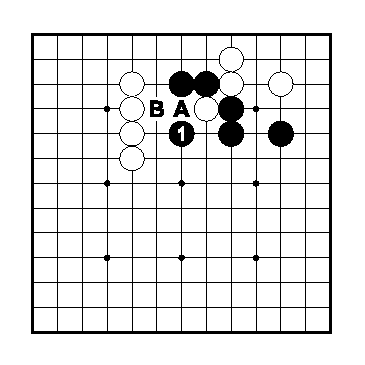
\includegraphics[width=1\textwidth]{7 - Problem 35 - Dia 1}
        \captionsetup{justification=centering}
        \caption*{\emph{Dia.\@~1. Correto}}
    \end{subfigure}
    \hspace{1cm}
    \begin{subfigure}[t]{.425\textwidth}
        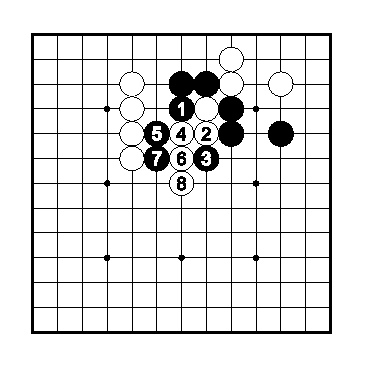
\includegraphics[width=1\textwidth]{7 - Problem 35 - Dia 2}
        \captionsetup{justification=centering}
        \caption*{\emph{Dia.\@~2. Errado}}
    \end{subfigure}
\end{figure}

Se Preto fizer atari com 1 no \emph{Dia.\@~2}, Branco estenderá em 2. Preto tentará contê-lo com 3 a 7, mas Branco escapa para o centro com 8.

\pagebreak

\subsubsection*{Resposta ao Problema 36}

Preto deveria jogar uma rede nas pedras brancas com 1 no \emph{Dia.\@~1}. Branco não escapará. Se Branco jogar 2, Preto bloqueia com 3, colocando as pedras brancas em um inescapável atari.

\begin{figure}[h!]
    \centering
    \begin{subfigure}[t]{.425\textwidth}
        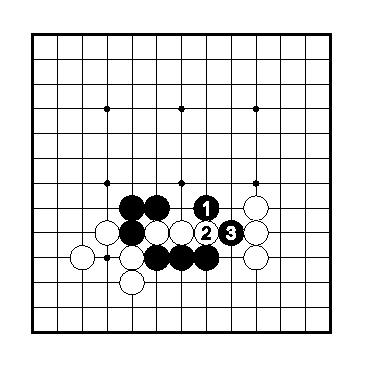
\includegraphics[width=1\textwidth]{7 - Problem 36 - Dia 1}
        \captionsetup{justification=centering}
        \caption*{\emph{Dia.\@~1. Correto}}
    \end{subfigure}
    \hspace{1cm}
    \begin{subfigure}[t]{.425\textwidth}
        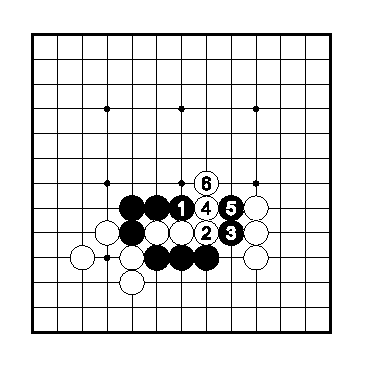
\includegraphics[width=1\textwidth]{7 - Problem 36 - Dia 2}
        \captionsetup{justification=centering}
        \caption*{\emph{Dia.\@~2. Errado}}
    \end{subfigure}
\end{figure}

Se Preto fizer atari com 1 no \emph{Dia.\@~1}, Branco estenderá para 2. Preto tenta contê-lo com 3 a 5, mas Branco escapa ao centro com 6.

\pagebreak

\subsubsection*{Resposta ao Problema 37}

Preto deveria jogar a rede de 1 nas pedras brancas no \emph{Dia.\@~1}. Branco não tem para onde fugir. Se ele estender para 2, Preto bloqueará com 3, e as pedras brancas estarão capturadas de qualquer maneira.

\begin{figure}[h!]
    \centering
    \begin{subfigure}[t]{.425\textwidth}
        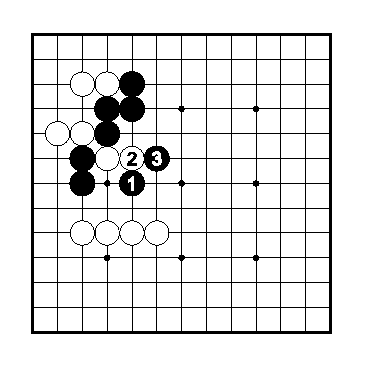
\includegraphics[width=1\textwidth]{7 - Problem 37 - Dia 1}
        \captionsetup{justification=centering}
        \caption*{\emph{Dia.\@~1. Correto}}
    \end{subfigure}
    \hspace{1cm}
    \begin{subfigure}[t]{.425\textwidth}
        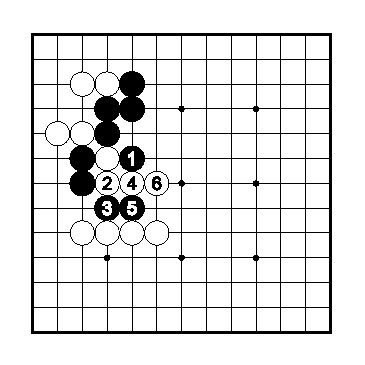
\includegraphics[width=1\textwidth]{7 - Problem 37 - Dia 2}
        \captionsetup{justification=centering}
        \caption*{\emph{Dia.\@~2. Errado}}
    \end{subfigure}
\end{figure}

Se Preto fizer atari com 1 no \emph{Dia.\@~2}, Branco estende em 2. Preto tentará contê-lo com 3 a 5, mas Branco escapa ao centro com 6.

\pagebreak

\subsubsection*{Resposta ao Problema 38}

Preto deveria enredar Branco com 1 no \emph{Dia.\@~1}. Branco não escapará. Se ele jogar \textbf{A}, Preto bloqueará em \textbf{B}, submetendo as pedras brancas a um atari sem escapatória.
    
Se Preto fizer atari com 1 e 3 no \emph{Dia.\@~2}, Branco estende com 2 e 4 e conecta suas pedras com aquelas à direita.

\begin{figure}[h!]
    \centering
    \begin{subfigure}[t]{.425\textwidth}
        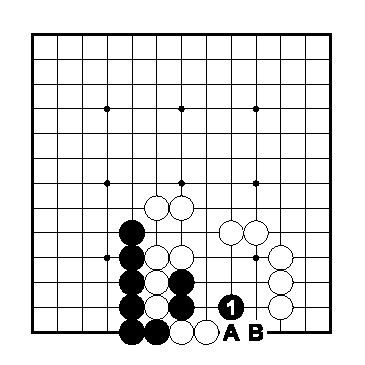
\includegraphics[width=1\textwidth]{7 - Problem 38 - Dia 1}
        \captionsetup{justification=centering}
        \caption*{\emph{Dia.\@~1. Correto}}
    \end{subfigure}
    \hspace{1cm}
    \begin{subfigure}[t]{.425\textwidth}
        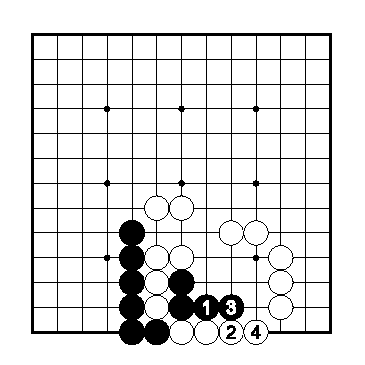
\includegraphics[width=1\textwidth]{7 - Problem 38 - Dia 2}
        \captionsetup{justification=centering}
        \caption*{\emph{Dia.\@~2. Errado}}
    \end{subfigure}
\end{figure}

Se Preto fizer atari com 1 e 3 no \emph{Dia.\@~2}, Branco estende com 2 e 4 e conecta suas pedras com aquelas à direita.

\pagebreak

\section{Táticas de Sacrifício}

Go abunda em termos de táticas de sacrifício que levam a capturas de pedras adversárias. Aqui seguem alguns exemplos.

\emph{Dia.\@~12.} Branco possui uma maneira de capturar as duas pedras marcadas, o que propiciará a conexão das quatro pedras no canto com aquelas isoladas no exterior.

\begin{figure}[h!]
    \centering
    \begin{subfigure}[t]{.31\textwidth}
        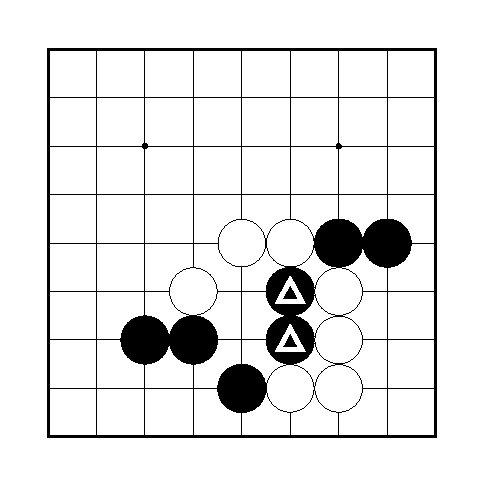
\includegraphics[width=1\textwidth]{7 - Sacrifice - Dia 12}
        \captionsetup{justification=centering}
        \caption*{\emph{Dia.\@~12}}
    \end{subfigure}
    \hspace{1cm}
    \begin{subfigure}[t]{.31\textwidth}
        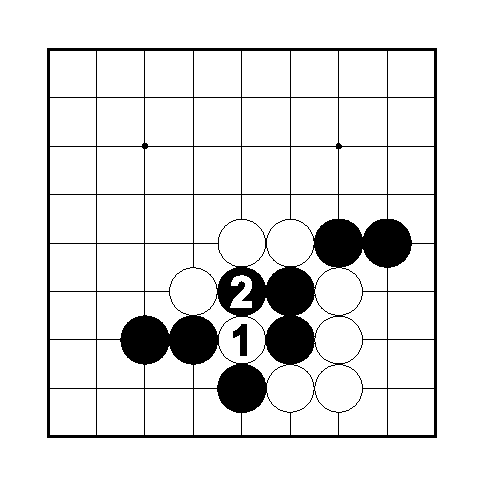
\includegraphics[width=1\textwidth]{7 - Sacrifice - Dia 13}
        \captionsetup{justification=centering}
        \caption*{\emph{Dia.\@~13}}
    \end{subfigure}
\end{figure}

\emph{Dia.\@~13.} Branco inicia o sacrifício com 1, colocando as duas pedras sob atari. Preto poderá capturar com 2.

\emph{Dia.\@~14.} Esse é o resultado. As três pedras marcadas estão em atari, então\ldots

\begin{figure}[h!]
    \centering
    \begin{subfigure}[t]{.31\textwidth}
        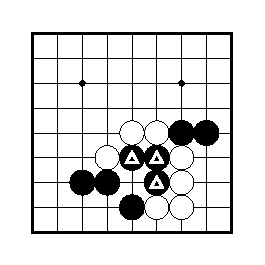
\includegraphics[width=1\textwidth]{7 - Sacrifice - Dia 14}
        \captionsetup{justification=centering}
        \caption*{\emph{Dia.\@~14}}
    \end{subfigure}
    \hspace{1cm}
    \begin{subfigure}[t]{.31\textwidth}
        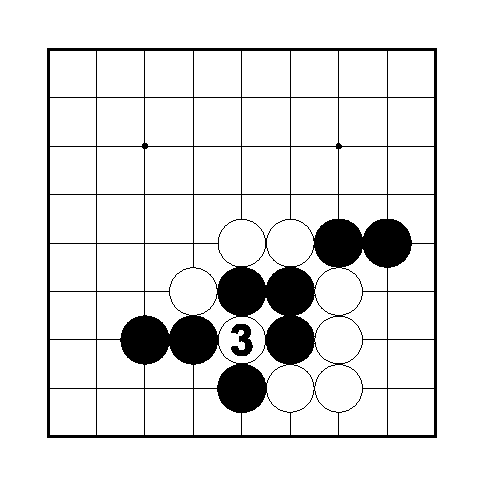
\includegraphics[width=1\textwidth]{7 - Sacrifice - Dia 15}
        \captionsetup{justification=centering}
        \caption*{\emph{Dia.\@~15}}
    \end{subfigure}
\end{figure}

\emph{Dia.\@~15.} Preto as captura com 3. Esse padrão, no qual um dos lados captura, e o outro recaptura, é denominado de \emph{ricochete}\footnote{Em inglês, o termo já é muito sedimentado, e é conhecido como \emph{snapback}.}.

\pagebreak

\emph{Dia.\@~16.} Como é que Preto poderia capturar as pedras brancas?

\begin{figure}[h!]
    \centering
    \begin{subfigure}[t]{.31\textwidth}
        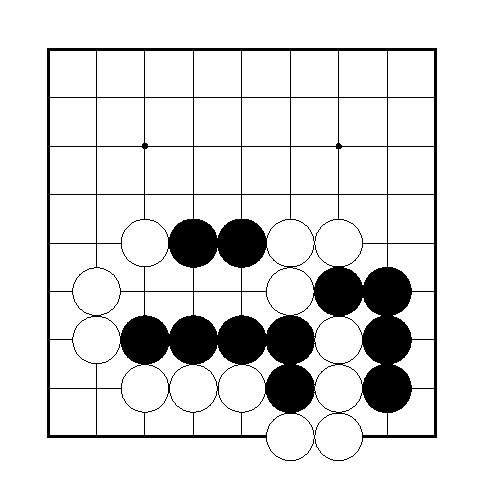
\includegraphics[width=1\textwidth]{7 - Sacrifice - Dia 16}
        \captionsetup{justification=centering}
        \caption*{\emph{Dia.\@~16}}
    \end{subfigure}
    \hfill
    \begin{subfigure}[t]{.31\textwidth}
        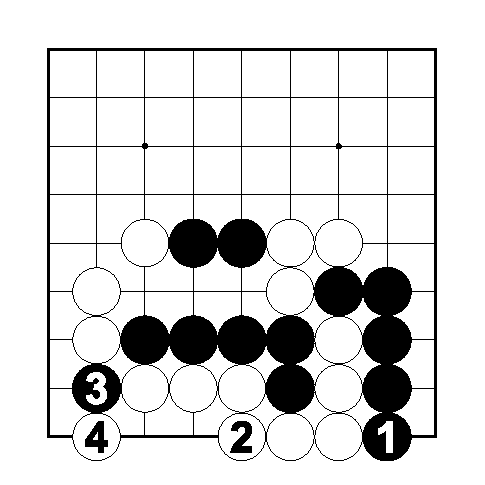
\includegraphics[width=1\textwidth]{7 - Sacrifice - Dia 17}
        \captionsetup{justification=centering}
        \caption*{\emph{Dia.\@~17}}
    \end{subfigure}
    \hfill
    \begin{subfigure}[t]{.31\textwidth}
        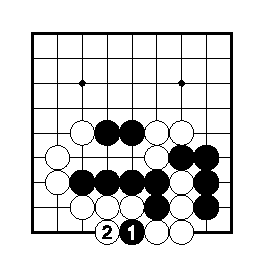
\includegraphics[width=1\textwidth]{7 - Sacrifice - Dia 18}
        \captionsetup{justification=centering}
        \caption*{\emph{Dia.\@~18}}
    \end{subfigure}
\end{figure}

\emph{Dia.\@~17.} Se Preto simplesmente fizer atari com 1, Branco conectará com 2. Se Preto cortar com 3, Branco fará atari com 4, e as pedras brancas não poderão ser capturadas.

\emph{Dia.\@~18.} Se Preto quiser capturar algumas pedras, ele terá de sacrificar uma com 1. Se Branco capturar com 2\ldots

\emph{Dia.\@~19.} Preto faz atari com 3. Se Branco conecta com 4, Preto corta com 5, colocando as nove pedras Brancas em atari. Branco não consegue evitar de ser capturado no próximo movimento. Ao invés de Branco 4\ldots

\begin{figure}[h!]
    \centering
    \begin{subfigure}[t]{.31\textwidth}
        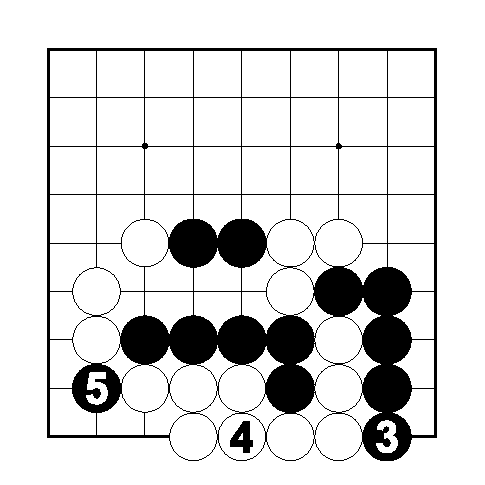
\includegraphics[width=1\textwidth]{7 - Sacrifice - Dia 19}
        \captionsetup{justification=centering}
        \caption*{\emph{Dia.\@~19}}
    \end{subfigure}
    \hfill
    \begin{subfigure}[t]{.31\textwidth}
        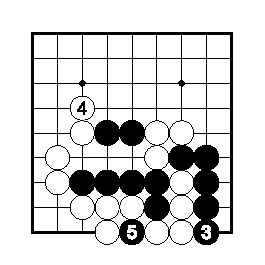
\includegraphics[width=1\textwidth]{7 - Sacrifice - Dia 20}
        \captionsetup{justification=centering}
        \caption*{\emph{Dia.\@~20}}
    \end{subfigure}
    \hfill
    \begin{subfigure}[t]{.31\textwidth}
        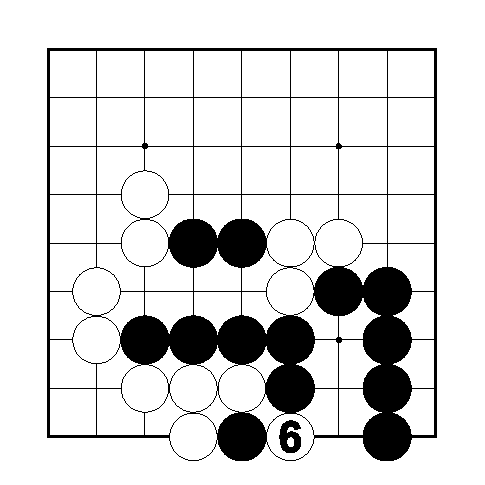
\includegraphics[width=1\textwidth]{7 - Sacrifice - Dia 21}
        \captionsetup{justification=centering}
        \caption*{\emph{Dia.\@~21}}
    \end{subfigure}
\end{figure}

\emph{Dia.\@~20.} Já que Branco não pode evitar de perder quatro pedras, ele não deveria defendê-las. Em seu lugar, ele deveria jogar jogar 4 em outro lugar. Quando Preto capturar com 5\ldots

\emph{Dia.\@~21.} Branco pode recapturar uma pedra com 6, desta maneira, limitando sua perda.

\pagebreak

\subsection{Problemas 39 a 46}

\begin{figure}[h!]
    \centering
    \begin{subfigure}[t]{.35\textwidth}
        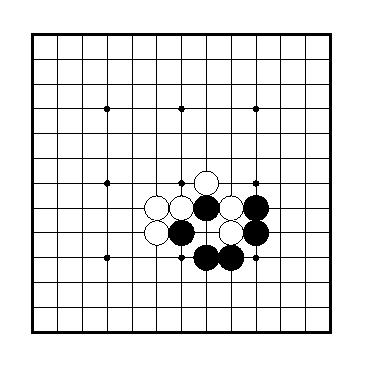
\includegraphics[width=1.25\textwidth]{7 - Problem 39}
        \captionsetup{margin={0in,0.15in}}
        \caption*{\textbf{Problema 39}: \emph{Como Preto pode capturar duas pedras?}}
    \end{subfigure}
    \hspace{1.5cm}
    \begin{subfigure}[t]{.35\textwidth}
        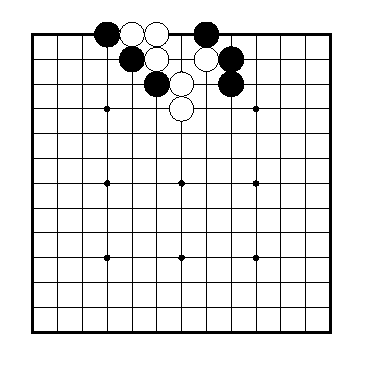
\includegraphics[width=1.25\textwidth]{7 - Problem 40}
        \captionsetup{margin={0in,.15in}}
        \caption*{\textbf{Problema 40}: \emph{Como Preto pode capturar três pedras?}}
    \end{subfigure}
    \par\bigskip
    \begin{subfigure}[t]{.35\textwidth}
        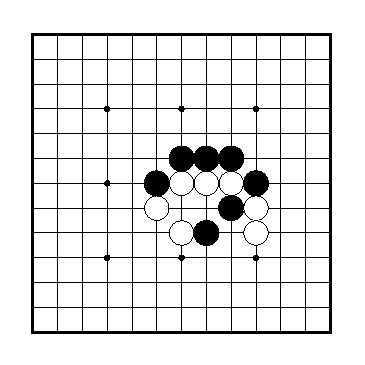
\includegraphics[width=1.25\textwidth]{7 - Problem 41}
        \captionsetup{margin={0in,.15in}}
        \caption*{\textbf{Problema 41}: \emph{Como Preto pode capturar três pedras?}}
    \end{subfigure}
    \hspace{1.5cm}
    \begin{subfigure}[t]{.35\textwidth}
        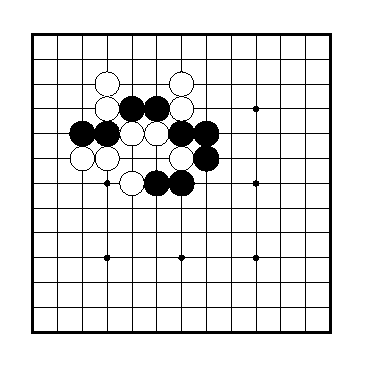
\includegraphics[width=1.25\textwidth]{7 - Problem 42}
        \captionsetup{margin={0in,.15in}}
        \caption*{\textbf{Problema 42}: \emph{Como Preto pode capturar três pedras?}}
    \end{subfigure}
\end{figure}

\pagebreak

\begin{figure}[h!]
    \centering
    \begin{subfigure}[t]{.35\textwidth}
        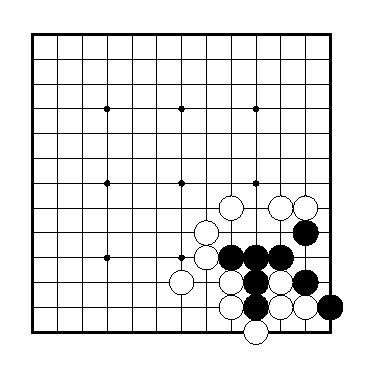
\includegraphics[width=1.25\textwidth]{7 - Problem 43}
        \captionsetup{margin={.15in,0in}}
        \caption*{\textbf{Problema 43}: \emph{Como Preto pode capturar três pedras?}}
    \end{subfigure}
    \hspace{1.5cm}
    \begin{subfigure}[t]{.35\textwidth}
        \includegraphics[width=1.25\textwidth]{7 - Problem 44}
        \captionsetup{margin={.15in,0in}}
        \caption*{\textbf{Problema 44}: \emph{Como Preto pode capturar seis pedras?}}
    \end{subfigure}
    \par\bigskip
    \begin{subfigure}[t]{.35\textwidth}
        \includegraphics[width=1.25\textwidth]{7 - Problem 45}
        \captionsetup{margin={.15in,0in}}
        \caption*{\textbf{Problema 45}: \emph{Como Preto pode conectar todas as suas pedras?}}
    \end{subfigure}
    \hspace{1.5cm}
    \begin{subfigure}[t]{.35\textwidth}
        \includegraphics[width=1.25\textwidth]{7 - Problem 46}
        \captionsetup{margin={.15in,0in}}
        \caption*{\textbf{Problema 46}: \emph{Como Preto pode conectar todas as suas pedras?}}
    \end{subfigure}
\end{figure}

\pagebreak

\subsection{Respostas aos Problemas 39 a 46}

\subsubsection*{Resposta ao Problema 39}

Preto deveria fazer atari nas duas pedras com 1 no \emph{Dia.\@~1}. Se Branco responder capturando a pedra marcada em \textbf{A}, Preto responderá jogando na pedra marcada e capturando três pedras.
    
\begin{figure}[h!]
    \centering
    \begin{subfigure}[t]{.425\textwidth}
        \includegraphics[width=1\textwidth]{7 - Problem 39 - Dia 1}
        \captionsetup{justification=centering}
        \caption*{\emph{Dia.\@~1. Correto}}
    \end{subfigure}
    \hspace{1cm}
    \begin{subfigure}[t]{.425\textwidth}
        \includegraphics[width=1\textwidth]{7 - Problem 39 - Dia 2}
        \captionsetup{justification=centering}
        \caption*{\emph{Dia.\@~2. Errado}}
    \end{subfigure}
\end{figure}

Se Preto defender a pedra em atari conectando em 1 no \emph{Dia.\@~2}, Branco conectará, e Preto não estará apto a capturar nenhuma pedra.

\pagebreak

\subsubsection*{Resposta ao Problema 40}

Preto deveria sacrificar uma pedra com 1 no \emph{Dia.\@~1}. Se Branco capturar em \textbf{A}, ele ainda estará sob atari, portanto Preto jogará de volta em 1, e capturará quatro pedras.

\begin{figure}[h!]
    \centering
    \begin{subfigure}[t]{.425\textwidth}
        \includegraphics[width=1\textwidth]{7 - Problem 40 - Dia 1}
        \captionsetup{justification=centering}
        \caption*{\emph{Dia.\@~1. Correto}}
    \end{subfigure}
    \hspace{1cm}
    \begin{subfigure}[t]{.425\textwidth}
        \includegraphics[width=1\textwidth]{7 - Problem 40 - Dia 2}
        \captionsetup{justification=centering}
        \caption*{\emph{Dia.\@~2. Errado}}
    \end{subfigure}
\end{figure}

Conectar com Preto 1 no \emph{Dia.\@~2} oferece a oportunidade de Branco consertar seu defeito em sua forma através da conexão em 2.

\pagebreak

\subsubsection*{Resposta ao Problema 41}

Preto deveria sacrificar uma pedra em 1 no \emph{Dia.\@~1}. Se Branco capturar em \textbf{A}, ele ainda estará sob atari, então Preto jogará de volta em 1 e capturará quatro pedras.
    
\begin{figure}[h!]
    \centering
    \begin{subfigure}[t]{.425\textwidth}
        \includegraphics[width=1\textwidth]{7 - Problem 41 - Dia 1}
        \captionsetup{justification=centering}
        \caption*{\emph{Dia.\@~1. Correto}}
    \end{subfigure}
    \hspace{1cm}
    \begin{subfigure}[t]{.425\textwidth}
        \includegraphics[width=1\textwidth]{7 - Problem 41 - Dia 2}
        \captionsetup{justification=centering}
        \caption*{\emph{Dia.\@~2. Errado}}
    \end{subfigure}
\end{figure}

Se Preto fizer atari com 1 no \emph{Dia.\@~2}, Branco conectará em 2, e Preto não conseguirá capturar nenhuma pedra.

\pagebreak

\subsubsection*{Resposta ao Problema 42}

Preto deveria sacrificar uma pedra com 1 no \emph{Dia.\@~1}. Se Branco capturar em \textbf{A}, ele ainda estará sob atari, e Preto jogará em 1 para capturar as quatro pedras.
    
\begin{figure}[h!]
    \centering
    \begin{subfigure}[t]{.425\textwidth}
        \includegraphics[width=1\textwidth]{7 - Problem 42 - Dia 1}
        \captionsetup{justification=centering}
        \caption*{\emph{Dia.\@~1. Correto}}
    \end{subfigure}
    \hspace{1cm}
    \begin{subfigure}[t]{.425\textwidth}
        \includegraphics[width=1\textwidth]{7 - Problem 42 - Dia 2}
        \captionsetup{justification=centering}
        \caption*{\emph{Dia.\@~2. Errado}}
    \end{subfigure}
\end{figure}

Se Preto capturar uma pedra com 1 no \emph{Dia.\@~2}, Branco conectará em 2. Agora, as quatro pedras marcadas não têm como escapar e serão capturadas.

\pagebreak

\subsubsection*{Resposta ao Problema 43}

Nenhum sacrifício é necessário. Preto deveria simplesmente fazer atari com 1 no \emph{Dia.\@~1}. Se Branco conectar em \textbf{A}, Preto capturará cinco pedras jogando em \textbf{B}. Se Branco conectar em \textbf{B}, Preto \textbf{A} capturará três pedras.
    
\begin{figure}[h!]
    \centering
    \begin{subfigure}[t]{.425\textwidth}
        \includegraphics[width=1\textwidth]{7 - Problem 43 - Dia 1}
        \captionsetup{justification=centering}
        \caption*{\emph{Dia.\@~1. Correto}}
    \end{subfigure}
    \hspace{1cm}
    \begin{subfigure}[t]{.425\textwidth}
        \includegraphics[width=1\textwidth]{7 - Problem 43 - Dia 2}
        \captionsetup{justification=centering}
        \caption*{\emph{Dia.\@~2. Errado}}
    \end{subfigure}
\end{figure}

Sacrificar uma pedra em 1 no \emph{Dia.\@~2} é um erro. Após os movimentos até Preto 5, Branco conectará em 1, e todas as suas pedras estarão seguras. Este exemplo demonstra que sacrifícios nem sempre funcionam\footnote{Especialmente quando próximos ao canto, em que as liberdades de cada pedra se comportam de maneiras mais peculiares.}.

\pagebreak

\subsubsection*{Resposta ao Problema 44}

Preto deveria fazer atari com 1 no \emph{Dia.\@~1}, sacrificando a pedra marcada. Se Branco capturar com 2, ele ainda estará em atari, então Preto jogará de volta onde a pedra marcada estava e capturará as sete pedras.
 
\begin{figure}[h!]
    \centering
    \begin{subfigure}[t]{.425\textwidth}
        \includegraphics[width=1\textwidth]{7 - Problem 44 - Dia 1}
        \captionsetup{justification=centering}
        \caption*{\emph{Dia.\@~1. Correto}}
    \end{subfigure}
    \hspace{1cm}
    \begin{subfigure}[t]{.425\textwidth}
        \includegraphics[width=1\textwidth]{7 - Problem 44 - Dia 2}
        \captionsetup{justification=centering}
        \caption*{\emph{Dia.\@~2. Errado}}
    \end{subfigure}
\end{figure}

Preto 1 no \emph{Dia.\@~1} também é atari, mas as pedras pretas possuem uma escassez de liberdades, então Branco conseguirá capturar três pedras com 2, e suas seis pedras estarão seguras.

\pagebreak

\subsubsection*{Resposta ao Problema 45}

Se Preto jogar 1 no \emph{Dia.\@~1}, Branco não consegue escapar do atari, já que possui falta de liberdades. Se ele conectar em \textbf{A}, Preto capturará as oito pedras jogando em \textbf{B}. Se Branco conectar em \textbf{B}, Preto capturará seis pedras jogando em \textbf{A}.
 
\begin{figure}[h!]
    \centering
    \begin{subfigure}[t]{.425\textwidth}
        \includegraphics[width=1\textwidth]{7 - Problem 45 - Dia 1}
        \captionsetup{justification=centering}
        \caption*{\emph{Dia.\@~1. Correto}}
    \end{subfigure}
    \hspace{1cm}
    \begin{subfigure}[t]{.425\textwidth}
        \includegraphics[width=1\textwidth]{7 - Problem 45 - Dia 2}
        \captionsetup{justification=centering}
        \caption*{\emph{Dia.\@~2. Errado}}
    \end{subfigure}
\end{figure}

Preto 1 no \emph{Dia.\@~2} é devagar demais. Branco conectará no ponto-chave de 2. Se Preto fizer atari em \textbf{A}, Branco resgata suas pedras conectando em \textbf{B}.

\pagebreak

\subsubsection*{Resposta ao Problema 46}

Se preto sacrificar em 1 no \emph{Dia.\@~1}, Branco precisará capturar em 2. Preto agora faz atari com 3. Se Branco conectar em 1, Preto captura seis pedras jogando em \textbf{A}. Se Branco conectar em \textbf{A}, Preto captura quatro pedras jogando em 1.
 
\begin{figure}[h!]
    \centering
    \begin{subfigure}[t]{.425\textwidth}
        \includegraphics[width=1\textwidth]{7 - Problem 46 - Dia 1}
        \captionsetup{justification=centering}
        \caption*{\emph{Dia.\@~1. Correto}}
    \end{subfigure}
    \hspace{1cm}
    \begin{subfigure}[t]{.425\textwidth}
        \includegraphics[width=1\textwidth]{7 - Problem 46 - Dia 2}
        \captionsetup{justification=centering}
        \caption*{\emph{Dia.\@~2. Errado}}
    \end{subfigure}
\end{figure}

Se Preto jogar qualquer outro movimento, em 1 no \emph{Dia.\@~2} por exemplo, Branco conectará em 2. Se Preto agora jogar em \textbf{A}, Branco conectará em \textbf{B}, e suas pedras estarão seguras. Entretanto, as pedras pretas ainda estão separadas.